Para acceder a sancionar a un solicitante se da click en el botón
	 \textbf{Gestionar Prestamos} localizado en la parte izquierda del menú de 
	 hamburguesa 
	
	\begin{figure}[hbtp]

	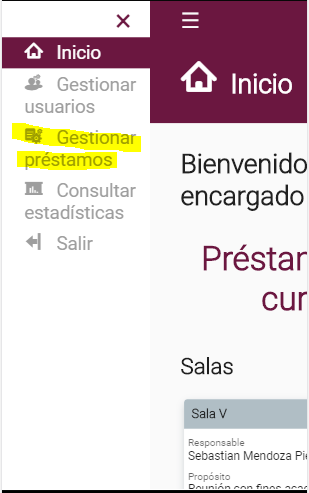
\includegraphics[scale=0.3]{images/InterfazMovil/IUGS07_bienvenida.PNG}
	\caption{Bienvenida}
	\end{figure}
Para iniciar el proceso de búsqueda de préstamos es necesario seleccionar el método de 
búsqueda a emplear, ya sea por: ID de préstamo o por fecha.

\subsection{Subpaso 1-A: Iniciar búsqueda por medio de ID}
\begin{enumerate}
	\item Seleccione el radio botón \textbf{Búsqueda por ID} en la interfaz
		\textbf{IUGS-17 Gestionar préstamos}.
		\begin{figure}[hbtp]
	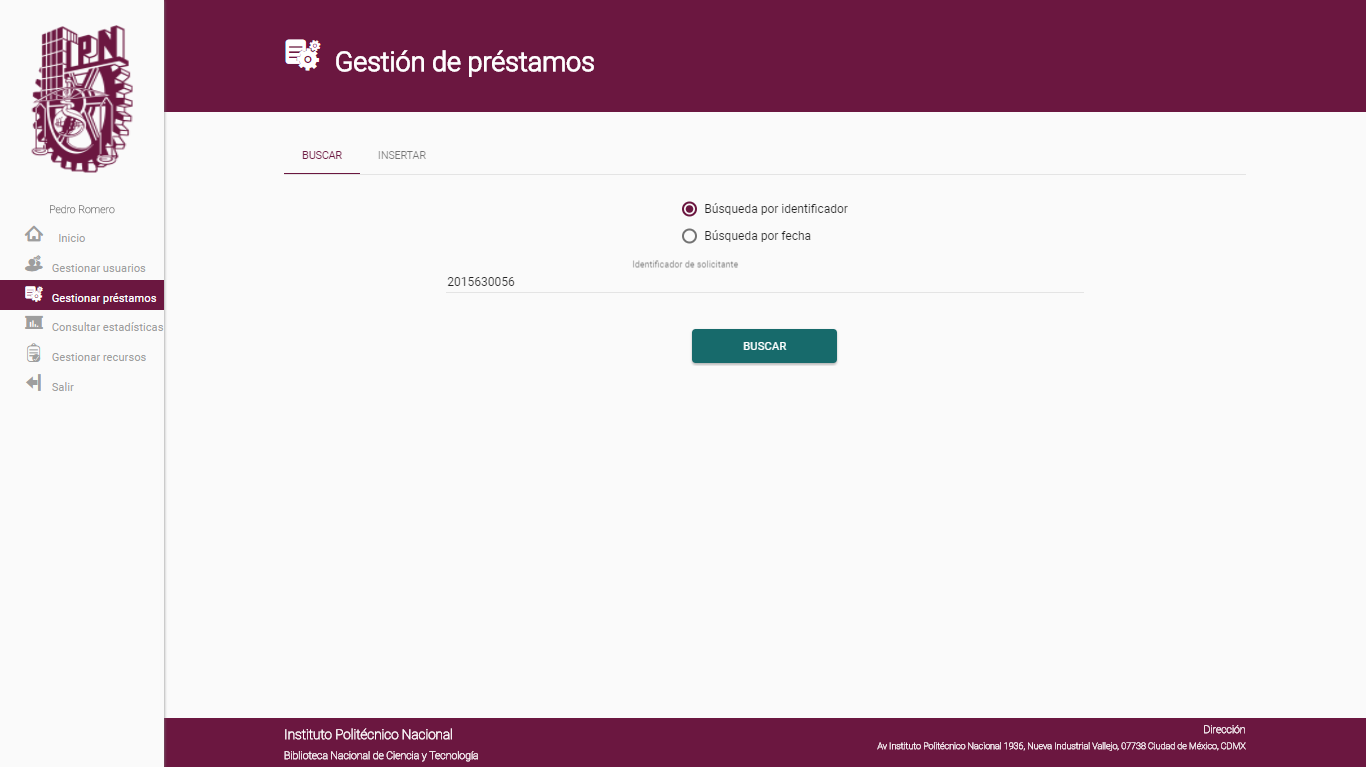
\includegraphics[scale=0.3]{images/InterfazMovil/IUGS07_gestionarPrestamoID.PNG}
	\caption{Gestionar Préstamo con Identificador}
	\end{figure}
	\item Ingrese el identificador a solicitar en el campo de texto.
	\item Presione el botón \textbf{Buscar}.
	
	
	\item Los resultados obtenidos son mostrados en la interfaz \textbf{IUGS-18 Préstamos encontrados}.
\end{enumerate}

\subsection{Subpaso 1-B: Iniciar búsqueda por medio de fecha}
\begin{enumerate}
	\item Seleccione el radio botón \textbf{Búsqueda por fecha} en la interfaz
		\textbf{IUGS-17 Gestionar préstamos}.
		\begin{figure}[hbtp]
	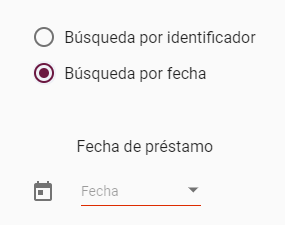
\includegraphics[scale=0.3]{images/InterfazMovil/IUGS07_gestionarPrestamoFecha.PNG}
	\caption{Gestionar Préstamo con Fecha}
	\end{figure}
	\item Seleccione la fecha a solicitar en el calendario mostrado.
	\item Presione el botón \textbf{Buscar}.
	\begin{figure}[hbtp]
	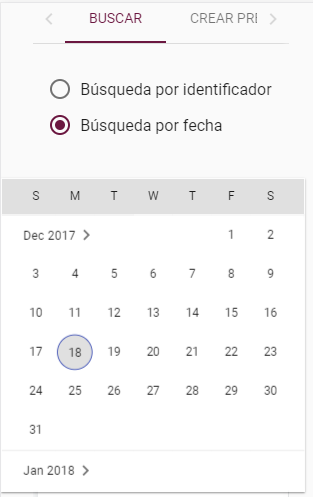
\includegraphics[scale=0.3]{images/InterfazMovil/IUGS07_gestionarPrestamoBuscar.PNG}
	\caption{Gestionar Préstamo Botón Buscar}
	\end{figure}
	\item Los resultados obtenidos son mostrados en la interfaz \textbf{IUGS-18 Préstamos encontrados}.
	\begin{figure}[hbtp]

	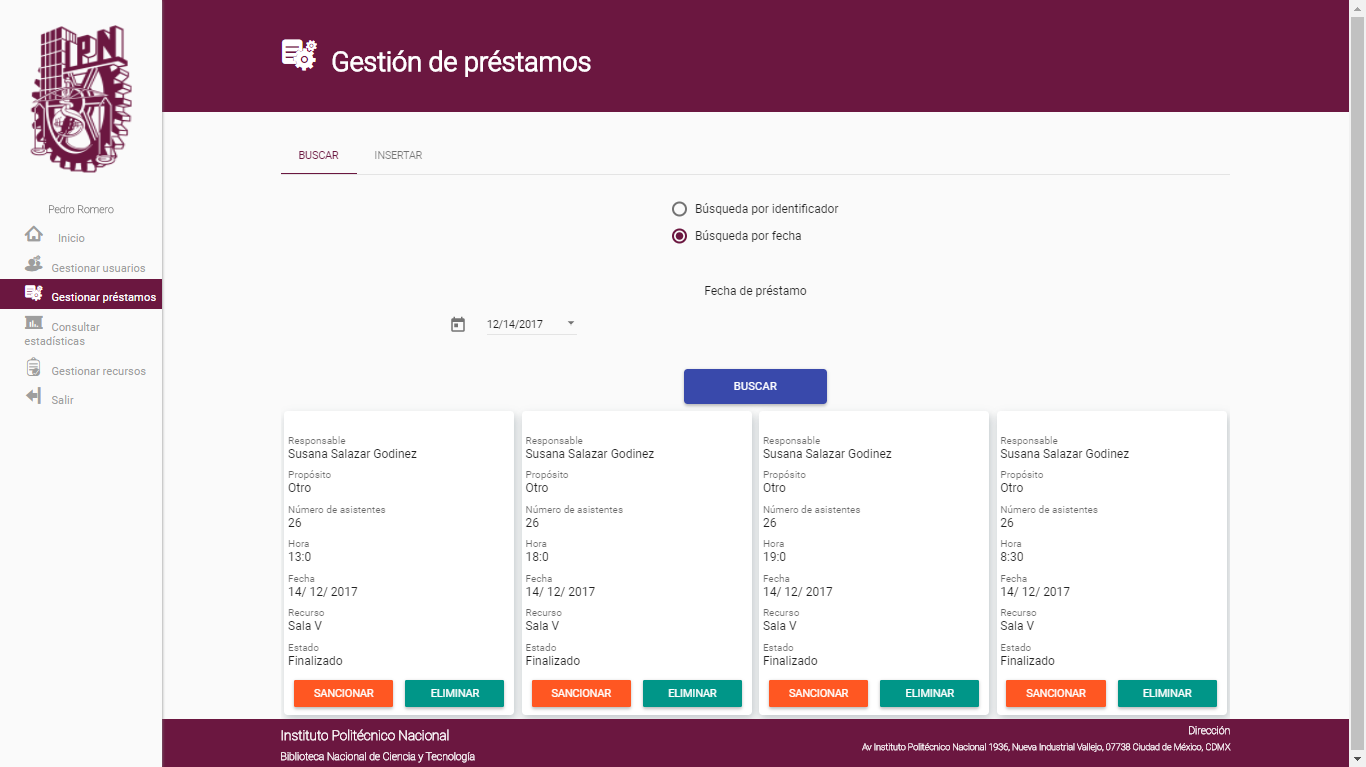
\includegraphics[scale=0.3]{images/InterfazMovil/IUGS07_busqueda.PNG}
	\caption{Busqueda Solicitante}
	\end{figure}
	
\end{enumerate}

